
\scsection{Введение в Технологию OSTIS}
\label{intro_ostis}

\begin{SCn}

\scnsectionheader{\currentname}

\scnstartsubstruct

\scnheader{Технология OSTIS}
\scnidtf{OSTIS}
\scnidtf{\uline{Открытая технология} проектирования \uline{совместимых} интеллектуальных систем}
\filemodetrue
\scnrelfromvector{предпосылки создания}{решение любой актуальной сложной (комплексной) задачи (понимание изображений, понимание текстов и речи, управление предприятиями и т.д.) требует комбинации в рамках системы различных \uline{видов знаний} (не только фактов, но и логических утверждений, ситуаций, событий, алгоритмов, т.д.) и различных \uline{моделей решения задач} (нейросетевых, логических, статистических моделей, классических алгоритмов и т.д.). При этом заранее нельзя сказать, какой именно набор понадобится для решения конкретной задачи.;
в настоящее время существуют системы, которые частично решают задачу интеграции различных моделей, однако такие системы делаются \uline{монолитными} и проектируются под \uline{конкретную задачу}. Разработка таких систем стоит огромных ресурсов, при этом развивать такие системы для решения других задач практически не представляется возможным, приходится делать все заново.}
\filemodefalse
\scnaddlevel{1}
\scnnote{В контексте \textit{Технологии OSTIS} мы считаем, что \uline{интеллектуальной} является не та система, которая может решить конкретную задачу (даже интеллектуальную), а та система, которая может легко \uline{обучаться} решению новых задач без существенных затрат.}
\scnaddlevel{-1}
\filemodetrue
\scnrelfromvector{принципы, лежащие в основе}{В основе \textit{Технологии OSTIS} лежит универсальный способ представления информации, названный \textit{SС-кодом}. В основу \textit{SC-кода} положены основные формализмы дискретной математики (теория множеств и теория графов), что обеспечивает как универсальность и унифицированность представления (можно представить любую информацию одинаковым образом), так и удобство обработки и восприятия человеком.;
Базовый \textit{Алфавит SC-кода} состоит всего из 5 элементов, на основе которых строятся все более сложные конструкции. При этом с помощью \textit{SC-кода} описываются не только знания системы, но и модели решения задач и даже интерфейс системы. Можно провести аналогию с тем, как из базового ограниченного набора элементарных частиц строятся различные вещества и далее различные объекты любой сложности.; 
Системы, построенные на основе \textit{Технологии OSTIS} (ostis-системы) состоят из \textit{базы знаний}, \textit{решателя задач} и \textit{интерфейса} взаимодействия с внешним миром (не обязательно пользовательского).;
\textit{База знаний ostis-системы} может описывать любые виды знаний, при этом легко дополняться новыми знаниями и новыми видами знаний.;
\textit{Решатель задач ostis-системы} основан на многоагентном подходе и позволяет легко интегрировать и комбинировать любые модели решения задач.;
\textit{Интерфейс ostis-системы} представляет собой совокупность специального вида \textit{базы знаний} и \textit{решателя задач}, т.е. также описывается средствами SC-кода.
}
\scnrelfromvector{преимущества}{В \uline{любую} ostis-систему без каких-либо \uline{накладных расходов} можно бесшовно \uline{интегрировать} любые \uline{знания} и \uline{модели решения задач} (по принципу plug\&play). Таким образом, не важно, что система умеет в данный момент, ее всегда можно переобучить на решение другой задачи.;
Разрабатываемые \uline{компоненты} ostis-систем \uline{универсальны} (могут использоваться в совершенно разных системах) и \uline{совместимы} между собой. Это означает, что можно накапливать \uline{библиотеку компонентов} и \uline{использовать компоненты повторно}, таким образом, сильно \uline{сокращается время разработки} каждой следующей системы. Например, в настоящее время универсальная часть (ядро) баз знаний позволяет сократить сроки разработки базы знаний новых систем на 40-60\%.;
За счет того, что вся система описывается средствами SC-кода, она может анализировать сама себя, искать в себе ошибки, оптимизировать собственную работу (обладает рефлексивностью). Рефлексивность считается одним из ключевых признаков интеллекта, даже люди далеко не всегда обладают рефлексивностью.;
За счет наличия базового \textit{Алфавита SC-кода} и возможности полного описания \textit{компьютерной системы} средствами \textit{SC-кода} возникает возможность сделать \textit{ostis-системы} полностью платформенно-независимыми (разделить модель системы и платформу интерпретации таких моделей). То есть разработка ostis-системы сводится к разработке ее модели и выполняется независимо не только от операционной системы, но и в принципе от архитектуры компьютера, на котором система работает. Платформа в свою очередь может быть реализована как \uline{программно} (наподобие виртуальной машины), так и \uline{аппаратно}.;
Как следует из предыдущего пункта, \textit{Технология OSTIS} является основной для нового типа компьютеров -- \uline{\textit{семантических компьютеров}}. В отличие от других компьютеров с нетрадиционной архитектурой (в том числе суперкомпьютеров), для которых не всегда понятно, как именно их использовать, для семантических компьютеров уже готова технология и конкретные системы, которые будут на них работать.;
За счет используемого в \textit{Технологии OSTIS} подхода к обработке информации (особого рода многоагентного подхода) ostis-системы оказываются изначально ориентированы на \uline{параллельную обработку информации}, в том числе, поддержку ее на аппаратном уровне (в рамках семантического компьютера).}
\filemodefalse
\scnaddlevel{1}
    \scntext{вывод}{Таким образом, по сравнению с традиционными технологиями, \textit{Технология OSTIS} позволяет при той же скорости обучения разработчиков и трудоемкости разработки новых компонентов значительно снизить сроки разработки систем за счет повторного использования компонентов и легкости их интеграции. При этом производительность \textit{ostis-системы} по сравнению с аналогичной традиционной системой в общем случае может оказаться ниже, но данная проблема будет решена при переходе на семантические компьютеры.

    При необходимости, \textit{ostis-система} может включать не только компоненты, разработанные на основе \textit{Технологии OSTIS}, но и легко интегрироваться с любыми другими системами и интегрировать другие компоненты посредством специального протокола обмена информацией и/или программного интерфейса (API). Такие компоненты не будут в полной мере обладать некоторыми важными свойствами ostis-систем (например, рефлексивностью) но это позволит заимствовать современные разработки и решить проблему производительности при решении наиболее ресурсоемких задач (например, при обучении нейросетей).
    }
\scnaddlevel{-1}
\scnnote{Важно отметить, что \uline{\textit{OSTIS} -- не конкретная интеллектуальная система} или способ решения задач какого-либо класса, это \uline{технология разработки интеллектуальных систем}, каждая из которых в свою очередь в каждый конкретный момент будет решать задачи определенного класса. При этом ключевые преимущества \textit{OSTIS} заключаются не в принципиально новых функциональных возможностях разрабатываемых систем (большинство \textit{ostis-систем} могут быть реализованы современными традиционными средствами), а в том, насколько легко можно \uline{модифицировать и развивать} разрабатываемые системы, адаптировать их под новые задачи, а также в том, насколько эффективно можно \uline{накапливать и использовать полученные компоненты} при разработке новых систем, снижая при этом сроки и трудоемкость их разработки.
}
\filemodetrue
\scnrelfromvector{текущий состав}{программная реализация платформы (модели семантического компьютера), которая лежит в основе каждой ostis-системы. Может использоваться как при разработке web-приложений, так и настольных и мобильных приложений.;
постоянно пополняемая \textit{Библиотека компонентов баз знаний ostis-систем}, включая универсальное \textit{Ядро баз знаний ostis-систем}. В текущий момент наличие данной библиотеки позволяет сократить сроки разработки баз знаний на 40-60\%.;
постоянно пополняемая \textit{Библиотека компонентов решателей задач ostis-систем}, включая механизмы поиска информации и некоторые модели решения задач, среди которых выделяется соответствующее \textit{Ядро решателей задач ostis-систем}. В настоящее время на первых этапах разработки системы оказывается достаточным использовать только \textit{Ядро решателей задач ostis-систем} и не разрабатывать дополнительно никаких компонентов.;
комплекс \textit{Средств информационной поддержки разработчиков ostis-систем} (включая описание самих моделей, а также методики и руководства), оформленных в виде интеллектуальной \textit{Метасистемы IMS.ostis} (IMS) и доступный онлайн \url{https://ims.ostis.net.}}

\scnrelfromvector{текущее применение}{на основе \textit{Технологии OSTIS} силами студентов и аспирантов активно развивается большое число открытых прототипов обучающих и справочных систем, которые можно найти на \url{https://github.com/ostis-apps};
разработки на основе \textit{Технологии OSTIS} успешно внедрены на ОАО ``Савушкин продукт''  при разработке системы информационного обслуживания сотрудников и при разработке компонентов систем контроля качества продукции;
\textit{Технология OSTIS} позволит значительно более эффективно реализовать анализ естественного языка (включая речь), в том числе для чат-ботов, синхронного перевода и речевых ассистентов. В настоящее время выполняется ряд проектов по данной тематике.}
\filemodefalse
\scntext{планы развития}{Предполагается, что в ближайшем будущем \textit{Метасистема IMS.ostis} и другие \textit{ostis-системы} будут объединены в распределенную облачную \textit{ostis-систему}, названную \textit{Экосистемой OSTIS}. Общая архитектура экосистемы показана на рисунке \textit{Архитектура Экосистемы OSTIS}. При этом все \textit{ostis-системы} в составе \textit{Экосистемы OSTIS} будут в каждый момент времени совместимы между собой, при этом совместимость будет контролироваться автоматически. Любой желающий сможет внести свой вклад в развитие любой из ostis-систем в составе \textit{Экосистемы OSTIS}, в первую очередь -- \textit{Метасистемы IMS.ostis}, при этом вклад будет автоматически верифицироваться и оцениваться. В то же время, как видно из представленной архитектуры, владельцы \textit{ostis-систем} смогут самостоятельно выбирать, какой частью своей информации они готовы поделиться с другими пользователями \textit{Экосистемы OSTIS}, персональная же часть информации будет гарантированно защищена.}

\scnheader{Архитектура Экосистемы OSTIS}
\scneqimage{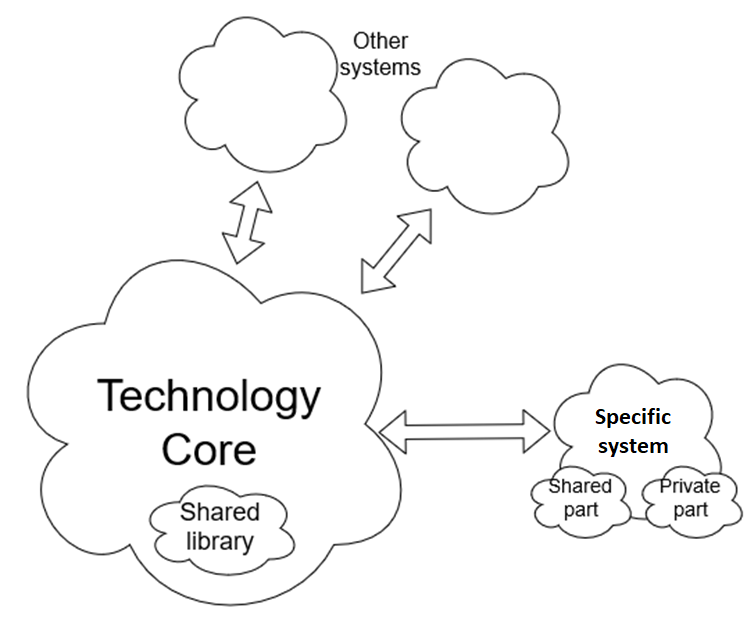
\includegraphics[width=0.6\textwidth]{figures/chapter0/ecosystem.png}}

\scnheader{Технология OSTIS}
\scnrelfromvector{текущие проекты}{Проект Экосистема OSTIS;Проект Метасистема IMS.ostis;Проект Семейство различных вариантов реализации универсального интерпретатора семантических моделей интеллектуальных систем\\
\scnaddlevel{1}
    \scnrelfromlist{подпроект}{Проект Программно реализованный на современных компьютерах универсальный интерпретатор семантических моделей интеллектуальных систем;Проект Семантический ассоциативный компьютер}
\scnaddlevel{-1}
;Проект Комплекс совместимых средств проектирования интеллектуальных систем\\
\scnaddlevel{1}
    \scnrelfromlist{подпроект}{Проект Встраиваемая типовая интеллектуальная система комплексной поддержки проектирования баз знаний;Проект Интеллектуальная система комплексной поддержки проектирования решателей задач интеллектуальных систем;Проект Интеллектуальная система комплексной поддержки проектирования вербальных интерфейсов интеллектуальных систем;Проект Интеллектуальная система комплексной поддержки проектирования невербальных интерфейсов}
\scnaddlevel{-1}
;Проект Семейство совместимых интеллектуальных справочных, обучающих и help-систем\\
\scnaddlevel{1}
    \scnrelfromlist{подпроект}{Проект Специализированные средства разработки совместимых интеллектуальных справочных, обучающих и help-систем различного назначения;Проект Комплекс семантически совместимых интеллектуальных справочных и обучающих систем по всем дисциплинам среднего образования;Проект Комплекс семантически совместимых интеллектуальных справочных и обучающих систем по всем дисциплинам, являющихся базовыми при подготовке инженеров по информационным специальностям;Проект Комплекс семантически совместимых интеллектуальных справочных и обучающих систем по всем специальным дисциплинам специальности ''Искусственный интеллект''{};Проект Семейство совместимых интеллектуальных справочных и обучающих систем по стандартам различного вида}
\scnaddlevel{-1}
;Проект Семейство совместимых интеллектуальных корпоративных систем ситуационного управления\\
\scnaddlevel{1}
    \scnrelfromlist{подпроект}{Проект Интеллектуальная корпоративная система ситуационного управления предприятием рецептурного производства;Проект Интеллектуальная корпоративная система ситуационного управления деятельностью выпускающей кафедры технического вуза}
\scnaddlevel{-1}
}
\scnrelfromvector{будущие проекты}{
Проект Семейство совместимых интеллектуальных систем автоматизации проектирования в различных областях;Проект Семейство совместимых порталов знаний\\
\scnaddlevel{1}
    \scnrelfrom{подпроект}{Проект Портал научных знаний по искусственному интеллекту}
\scnaddlevel{-1}
;Проект Семейство совместимых интеллектуальных систем экскурсионного обслуживания;Проект Семейство совместимых интеллектуальных геоинформационных систем;Проект Семейство совместимых интеллектуальных робототехнических систем и специализированных средств их разработки;Проект Семейство совместимых интеллектуальных систем персонального обслуживания и мониторинга\\
\scnaddlevel{1}
    \scnrelfromlist{подпроект}{Проект Интеллектуальная система персонального обслуживания и мониторинга пользователей и разработчиков компьютерных систем, входящих в Экосистему OSTIS;Проект Интеллектуальный персональный ассистент по взаимодействию с традиционными internet-системами и их пользователями;Проект Интеллектуальная система персонального комплексного медицинского мониторинга и контроля}
\scnaddlevel{-1}
}

\scnsegmentheader{Понятие ostis-технологии}
\scnstartsubstruct

\scnheader{ostis-технология}
\scnreltoset{объединение}{
ostis-технология проектирования\\
\scnaddlevel{1}
	\scnsubdividing{
		ostis-технология проектирования ostis-систем соответствующего класса\\
		\scnaddlevel{1}
			\scnhaselement{Базовая ostis-технология проектирования ostis-систем}
		\scnaddlevel{-1}
		;ostis-технология проектирования соответствующего класса компонентов ostis-систем\\
		\scnaddlevel{1}
			\scnhaselement{Базовая ostis-технология проектирования баз знаний ostis-систем}
			\scnhaselement{Базовая ostis-технология проектирования решателей задач ostis-систем}
			\scnhaselement{Базовая ostis-технология проектирования интерфейсов ostis-систем}
		\scnaddlevel{-1}
		;ostis-технология проектирования объектов заданного класса, не являющихся ostis-системами\\
	}
\scnaddlevel{-1}
;ostis-технология производства\\
\scnaddlevel{1}
	\scnsuperset{технология производства спроектированных ostis-систем}
	\scnsuperset{ostis-технология управления производством спроектированных продуктов заданного класса, не являющихся ostis-системами}
\scnaddlevel{-1}
;технология эксплуатации ostis-систем\\
\scnaddlevel{1}
	\scnhaselement{Базовая технология эксплуатации ostis-систем}
	\scnsuperset{технология эксплуатации ostis-систем соответствующего класса}
	\scnaddlevel{1}
		\scnsuperset{ostis-технология управления производством спроектированных продуктов заданного класса, не являющихся ostis-системами}
		\scnaddlevel{1}
			\scnidtf{технология эксплуатации ostis-систем управления производством спроектированных продуктов заданного класса, не являющихся ostis-системами}
			\scnaddlevel{-1}
	\scnaddlevel{-1}
\scnaddlevel{-1}
;технология реинжиниринга ostis-систем\\
\scnaddlevel{1}
	\scnhaselement{Базовая технология реинжиниринга ostis-систем}
	\scnsuperset{технология реинжиниринга ostis-систем соответствующего класса}
\scnaddlevel{-1}
}

\scnheader{ostis-технология}
\scnidtf{компонент Технологии OSTIS}
\scnhaselement{Ядро Технологии OSTIS}
\scnaddlevel{1}
	\scnidtf{Базовая ostis-технология}
\scnaddlevel{-1}
\scnsuperset{частная ostis-технология}
\scnaddlevel{1}
	\scnsuperset{ostis-технология проектирования соответствующего класса компонентов ostis-систем}
	\scnaddlevel{1}
		\scnhaselement{Технология проектирования баз знаний ostis-систем}
		\scnhaselement{Технология проектирования решателей задач ostis-систем}
		\scnhaselement{Технология проектирования невербальных интерфейсов ostis-систем с внешней средой}
		\scnhaselement{Технология проектирования интерфейсов ostis-систем с другими техническими системами}
		\scnhaselement{Технология проектирования пользовательских интерфейсов ostis-систем}
	\scnaddlevel{-1}
\scnaddlevel{-1}
\scnsuperset{специализированная ostis-технология проектирования ostis-систем соответствующего класса}
\scnaddlevel{1}
	\scnhaselement{Технология проектирования ostis-систем управления предприятиями рецептурного производства}
	\scnhaselement{Технология проектирования ostis-систем управления предприятиями производства молочной продукции}
	\scnhaselement{Технология проектирования интеллектуальных обучающих ostis-систем}
	\scnhaselement{Технология проектирования интеллектуальных обучающих ostis-систем для школьников}
	\scnhaselement{Технология проектирования интеллектуальных обучающих ostis-систем для подготовки специалистов в области Математики}
	\scnhaselement{Технология проектирования интеллектуальных обучающих ostis-систем для подготовки специалистов в области Искуственного интеллекта}
\scnaddlevel{-1}

\scnheader{ostis-технология проектирования}
\scnnote{Каждой ostis-технологии проектирования соответсвует своя ostis-система автоматизации проектирования соответствующего класса объектов}
\scnrelfrom{соответствующее семейство средств автоматизации}{ostis-система автоматизации проектирования}
\scnrelfrom{соответствующее семейство классов проектируемых объектов}{{\normalfont(}ostis-система автоматизации проектирования ostis-систем $\cup$ ostis-система автоматизации проектирования объектов, не являющихся ostis-системами{\normalfont)}}
\scnsuperset{ostis-технология проектирования ostis-систем соответствующего класса}

\scnheader{ostis-технология проектирования ostis-систем соответствующего класса}
\scnidtf{технология проектирования \textit{ostis-систем} соответствующего (заданного) класса, который, в свою очередь, соответствует определенному \textit{виду человеческой деятельности}, подвиды которого автоматизируются с помощью указанных выше проектируемых \textit{ostis-систем}}

\scnheader{ostis-технология}
\scnrelfromlist{отношение, заданное на данном множестве}{частная технология*; специализированная технология*; комплекс специализированных технологий*}
\scnidtf{Базовая частная или специализированная технология, входящая в состав комплексной \textit{Технологии OSTIS}, которая:
\begin{scnitemize}
	\item направлена на автоматизацию конкретного вида человеческой деятельности;
	\item ориентирована на использование ostis-систем (как индивидуальных, так и коллективных) в качестве самостоятельных субъектов или активных интеллектуальных инструментов, либо на использование человеко-машинных ostis-сообществ при решении:
	\begin{scnitemizeii}
		\item как задач, выполняемых в памяти ostis-систем (в т.ч. в памяти коллективов ostis-систем);
		\item так и задач, выполняемых во внешней среде ostis-систем, в процессе решения которых субъектами соответствующих действий либо ostis-системы (индивидуальные или коллективные), либо конкретные персоны, либо ostis-сообщества.
	\end{scnitemizeii}
\end{scnitemize}
}
\scnidtf{Множество всевозможных технологий, соответствующих стандартам технологии OSTIS и направленных на автоматизацию различных конкретных видов человеческой деятельности}
\scnrelboth{следует отличать}{Технология OSTIS}
\scnaddlevel{1}
 	\scnnote{\textit{Технология OSTIS} в отличие от понятия \textit{ostis-технологии} представляет собой не множество технологий, а комплекс взаимосвязанных между собой самых различных технологий, превращающий указанное множество технологий в единую объединенную технологию, в сумму взаимосвязанных глубоко интегрированных технологий. В этом смысле Технология OSTIS является максимальной ostis-технологией, в состав которой входят все ostis-технологии.}
\scnaddlevel{-1}
\scnreltoset{включение;пример}{
ostis-технология проектирования и перепроектирования;
ostis-технология производства;
ostis-технология публикации и согласования результатов научно-технической деятельности (в широком смысле);
ostis-технология образования}
\scnreltoset{включение;пример}{
Технология OSTIS;
OSTIS-технология проектирования, реализации и реинжиниринга ostis-систем;
OSTIS-технология разработки стандартов Технологии OSTIS}

\scnheader{ostis-технология коллективной разработки информационных ресурсов (различного вида)}
\scnsuperset{ostis-технология коллективного проектирования}
\scnsuperset{ostis-технология коллективной разработки планов}
\scnsuperset{ostis-технология публикации и согласования результатов научно-технической деятельности}
\scnsubset{ostis-технология}

\scnheader{ostis-технология эксплуатации ostis-систем}
\scnidtf{Общие методы и средства (языковые и интерфейсные) организации взаимодействия ostis-систем со своими конечными пользователями}
\scnsubset{ostis-технология}
\scnnote{Поскольку в рамках Экосистемы OSTIS каждому человеку придется взаимодействовать с больщим числом ostis-систем разного назначения, принципы организации взаимодействия всех ostis-систем со своими пользователями должны быть абсолютно одинаковыми. Удобство (usability) пользовательских интерфейсов должно быть направлено не только на синтаксическую красоту, но и на простую семантическую интерпретацию (понятность).}

\scnheader{ostis-технология проектирования ostis-систем}
\scnidtf{Технология построения (разработки) логико-семантических моделей (sc-моделей) ostis-систем}
\scniselement{ostis-технология}
\scnnote{Продуктом каждого завершенного (целостного) коллективного проекта, реализованного в рамках этой технологии, является полная \textit{логико-семантическая модель ostis-системы}.}
\scnrelfrom{класс продуктов}{логико-семантическая модель ostis-системы}
\scnrelfrom{средство}{Метасистема IMS OSTIS}
\scnrelfrom{класс субъектов}{коллектив разработчиков ostis-системы}
\scnrelfrom{класс исходных данных}{исходная спецификация ostis-системы}

\scnheader{ostis-технология реализации ostis-систем}
\scnidtf{Технология сборки и установки ostis-систем}
\scniselement{ostis-технология}
\scnrelfrom{исходная информация}{логико-семантическая модель ostis-системы}
\scnrelfrom{комплектация}{универсальный интерпретатор логико-семантических моделей ostis-систем}
\scnaddlevel{1}
	\scnnote{Это, своего рода, "мотор"{}, "движок"{} ostis-систем}
\scnaddlevel{-1}
\scnrelfrom{методы}{Методика реализации ostis-систем}
\scnrelfrom{активный инструмент}{Метасистема IMS OSTIS}
\scnrelfrom{продукты}{ostis-система}

\scnheader{ostis-технология обновления ostis-систем}
\scnidtf{Технология реинжирования (перепроектирования) ostis-систем в ходе их эксплуатации}
\scniselement{ostis-технология}
\scnheader{следует отличать*}
\scnhaselementset{Технология обновления ostis-систем; Технология проектирования ostis-систем}
\scnaddlevel{1}
	\scnnote{Эти технологии сходны. Их методы и средства совпадают. Не совпадают только исходные данные и результаты, которыми в \textit{Технологии обновления ostis-систем} являются предшествующие и последующие состояния ostis-систем. В \textit{Технологии проектирования ostis-систем} исходными данными являются исходные спецификации (замыслы) проектируемых ostis-систем, и результатами -- полные логико-семантические модели этих систем}
\scnaddlevel{-1}

\scnheader{Технология OSTIS}
\scnidtf{Совокупность (интеграция, объединение) всех ostis-технологий}
\scnrelto{интеграция}{ostis-технология}
\scnidtf{Комплекс (множество) семантически совместимых \textit{технологий}, в состав которого входит \textit{Ядро Технологии OSTIS} и иерархическая система \textit{ostis-технологий}, каждая из которых ориентирована на \textit{проектирование}, \textit{производство}, \textit{эксплуатацию} или \textit{реинжиниринг} соответствующего \textit{класса ostis-систем}, обеспечивающих автоматизацию соответствующего \textit{вида человеческой деятельности}. При этом каждая такая проектируемая \textit{ostis-система} автоматизирует либо область, либо \textit{вид человеческой деятельности}, которая (который) является соответственно либо экземпляром (элементом), либо подвидом (подклассом) указанного выше \textit{вида человеческой деятельности}, соответствующего используемой \textit{специализированной ostis-технологии}.}

%стр 197 уточнить ключевой элемент (неролевое или ролевое?)
\scnheader{Ядро Технологии OSTIS}
\scnidtf{Универсальная базовая \textit{ostis-технология}}
\scnidtf{Универсальный компонент Технологии OSTIS}

\scniselementrole{ключевой элемент}{ostis-технология}
\scnrelto{ядро}{Технология OSTIS}
\scnhaselement{технология}
\scnrelfrom{вид деятельности, выполняемой с помощью технологии}{проектирование, производство, эксплуатация и реинжиниринг ostis-системы}
\scnaddlevel{1}
	\scnreltoset{объединение}{
		проектирование ostis-системы\\
		\scnaddlevel{1}
			\scnidtf{построение логико-семантической модели ostis-системы}
		\scnaddlevel{-1}
		;производство ostis-системы\\
		\scnaddlevel{1}
			\scnidtf{сборка логико-семантической модели ostis-системы и загрузка этой модели в память универсального интерпретатора таких моделей}
		\scnaddlevel{-1}
		;эксплуатация ostis-системы\\
		\scnaddlevel{1}
			\scnidtf{базовый (предметно-независимый) уровень организации деятельности конечного пользователя ostis-системы с помощью соответствующих методов	и средств}
		\scnaddlevel{-1}
		;реинжиниринг ostis-системы\\
		\scnaddlevel{1}
			\scnidtf{совершенствование ostis-системы в процессе её эксплуатации}
		\scnaddlevel{-1}
	}
	\scnrelfrom{создаваемые продукты}{ostis-система\\
		\scnidtf{\textit{интеллектуальная компьютерная система}, построенная в соответствии со стандартом \textit{Технологии OSTIS}, предъявляемым к продуктам, создаваемым с помощью этой технологии}
		\scnaddlevel{1}
			\scnnote{Указанный стандарт продуктов, создаваемых с помощью технологии OSTIS есть не что иное, как \textit{общая формальная семантическая теория интеллектуальных компьютерных систем}}
		\scnaddlevel{-1}
	}
\scnaddlevel{-1}
\scnrelfromlist{частная технология}{
	Базовая Технология Проектирования ostis-систем\\
	\scnaddlevel{1}
		\scnrelfromlist{частная технология}{
			Технология проектирования баз знаний ostis-систем\\
			;Технология проектирования решателей задач ostis-систем\\
			;Технология проектирования интерфейсов ostis-систем\\
			\scnrelfromlist{частная технология}{
				Технология проектирования невербальных интерфейсов ostis-систем с внешней средой\\
				;Технология проектирования интерфейсов ostis-систем с другими техническими системами\\
				;Технология проектирования пользовательских интерфейсов ostis-систем
			}
		}
		\scnrelfrom{реализация}{Метасистема IMS.ostis}
		\scnaddlevel{1}
			\scnidtf{Intelligent MetaSystem for ostis-systems design}
			\scnidtf{OSTIS-система автоматизации проектирования ostis-систем}
		\scnaddlevel{-1}
	\scnaddlevel{-1}
	;Технология производства ostis-систем\\
	\scnaddlevel{1}
		\scnexplanation{Основным компонентом, точнее, инструментальным средством \textit{технологии производства ostis-систем} является \textit{универсальный интерпретатор логико-семантических моделей ostis-систем}. Указанные \textit{логико-семантические модели ostis-систем} являются результатом \textit{проектирования ostis-систем} и представляют собой начальные (исходные) состояния \textit{баз знаний} разрабатываемых \textit{ostis-систем}. В отличие от \textit{инструмента производства ostis-систем}, методика их производства весьма проста и сводится к сборке разработанных логико-семантических моделей (начального состояния \textit{баз знаний}) разрабатываемых \textit{ostis-систем} и загрузке этих моделей в память \textit{универсального интерпретатора логико-семантических моделей ostis-систем}.}
		\scnrelfrom{реализация}{универсальный интерпретатор логико-семантических моделей ostis-систем}
		\scnaddlevel{1}
			\scnexplanation{Такой интерпретатор логико-семантических моделей ostis-систем может быть реализован либо программно на \textit{современных компьютерах}, либо аппаратно в виде компьютеров нового поколения, ориентированных на реализацию интеллектуальных компьютерных систем.}
			\scnexplanation{С формальной точки зрения универсальный интерпретатор логико-семантических моделей ostis-систем является "пустой"{} ostis-системой, способной только на приём формализованной информации и её запись в свою память.}
		\scnaddlevel{-1}
	\scnaddlevel{-1}
	;Базовая технология эксплуатации ostis-систем\\
	\scnaddlevel{1}
		\scnidtf{Общая технология эксплуатации ostis-систем, включающая в себя общие методы и средства, используемые в процессе эксплуатации любых ostis-систем}
		\scnrelfrom{реализация}{встраиваемая ostis-система поддержки эксплуатации ostis-систем}
		\scnaddlevel{1}
			\scnexplanation{Данная ostis-система входит (интегрирована) в состав каждой ostis-системы.}
		\scnaddlevel{-1}
	\scnaddlevel{-1}
	;Базовая технология реинжиниринга ostis-систем\\
	\scnaddlevel{1}
		\scnrelfrom{реализация}{встраиваемая ostis-система поддержки реинжиниринга ostis-систем}
		\scnaddlevel{1}
			\scnexplanation{Данная ostis-система входит (интегрирована) в состав каждой ostis-системы и обеспечивает внесение изменений "руками"{} инженеров, сопровождающих эксплуатацию ostis-системы, или авторов базы знаний этой ostis-системы в текущее состояние базы знаний ostis-системы в ходе её экспуатации}
		\scnaddlevel{-1}
	\scnaddlevel{-1}
}
\scnrelfromlist{специализированная технология}{
	Общая технология проектирования ostis-систем автоматизации проектирования\\
	\scnaddlevel{1}
		\scnrelfromlist{специализированная технология}{
		Технология проектирования ostis-систем автоматизации проектирования строительных объектов\\
		;Технология проектирования ostis-систем автоматизации проектирования автомобилей\\
		;Технология проектирования ostis-систем автоматизации проектирования интегральных микросхем
		}
	\scnaddlevel{-1}
	;Технология проектирования ostis-систем управления производством\\
	\scnaddlevel{1}
		\scnrelfromlist{специализированная технология}{
		Технология проектирования ostis-систем управления строительством различных объектов\\
		;Технология проектирования ostis-систем управления производством автомобилей\\
		;Технология проектирования ostis-систем управления производством микросхем\\
		;Технология проектирования ostis-систем управления предприятиями рецептурного производства\\
		\scnaddlevel{1}
			\scnrelfrom{специализированная технология}{				Технология проектирования ostis-систем управления предприятиями производства молочной продукции}
		\scnaddlevel{-1}
		}
	\scnaddlevel{-1}
	;Технология проектирования интеллектуальных обучающих ostis-систем\\
	\scnaddlevel{1}
		\scnrelfromset{комплекс специализированных технологий}{
		Технология проектирования интеллектуальных обучающих ostis-систем для школьников\\
		;Технология проектирования интеллектуальных обучающих ostis-систем для студентов по общеобразовательным дисциплинам\\
		;Технология проектирования интеллектуальных обучающих ostis-систем для студентов по профильным дисциплинам\\
		;Технология проектирования интеллектуальных обучающих ostis-систем для магистрантов
		}
		\scnrelfromset{комплекс специализированных технологий}{
		Технология проектирования интеллектуальных обучающих ostis-систем по Математике\\
		;Технология проектирования интеллектуальных обучающих ostis-систем по Искусственному интеллекту
		}
		\scnnote{При проектировании конкретной обучающей ostis-системы необходимо использовать сразу две ostis-технологии...}
	\scnaddlevel{-1}
}

\scnheader{специализированная ostis-технология}
\scnnote{Приведённый нами перечень \textit{специализированных ostis-технологий} охватывает только некоторые области (фрагменты) \textit{человеческой деятельности}, подлежащие автоматизации с помощью \textit{ostis-технологий} в рамках \textit{Экосистемы OSTIS}.}

\scnheader{Ядро Технологии OSTIS}
\scnnote{Форма реализации \textit{Ядра Технологии OSTIS} (в виде ostis-системы \textit{IMS.ostis}) позволяет:
\begin{scnitemize}
	\item использовать достоинства \textit{Технологии OSTIS} для повышения уровня автоматизации развития самой \textit{Технологии OSTIS} и для существенного повышения темпов такого развития;
	\item приобрести очень важный опыт применения \textit{Технологии OSTIS};
	\item создать центрально ядро \textit{Экосистемы OSTIS}, обеспечивающее поддержку семантической совместимости всех \textit{ostis-систем} и \textit{ostis-сообществ}, входящих в состав \textit{Экосистемы OSTIS}.
\end{scnitemize}
}

\scnendstruct
\scninlinesourcecommentpar{Завершили рассмотрение \textit{понятия ostis-технологии}}

\scnendstruct

\end{SCn}
